%\documentclass[aps,prl,twocolumn,reprint,amsmath,amssymb]{revtex4-1}
\documentclass[10pt,amsmath,twocolumn,aps,prl,superscriptaddress,floatfix]{revtex4-1}
\usepackage{epsfig,color,graphicx}
\usepackage[T1]{fontenc}
\begin{document}
\newcommand{\Ang}{\ensuremath{\mathring{\text{A}}}}
\newcommand{\ltwid}{\mathrel{\raise.3ex\hbox{$<$\kern-.75em\lower1ex\hbox{$\sim$}}}}
\newcommand{\gtwid}{\mathrel{\raise.3ex\hbox{$>$\kern-.75em\lower1ex\hbox{$\sim$}}}}
\newcommand{\ket}[1]{\ensuremath{\vert #1 \rangle}}
\newcommand{\bra}[1]{\ensuremath{\langle #1 \vert}}
\newcommand{\braket}[2]{\ensuremath{\langle #1 \vert #2 \rangle}} % bra-ket inner product
\newcommand{\ketbra}[2]{\ensuremath{\vert #1 \rangle \langle #2 \vert}} % ket-bra outer product
\newcommand{\op}[1]{\ensuremath{\hat{#1}}} % operator
%\newcommand{\sill}{\psi_\mathrm{SILL}}
\newcommand{\sill}{\psi}
\newcommand{\trace}{{\rm Tr}}
\newcommand{\ntilde}{\tilde{n}}
\newcommand{\stilde}{\tilde{s}}
\newcommand{\atilde}{\tilde{\alpha}}
\newcommand{\new}{\color{red}}
\newcommand{\old}{\color{black}}
\newcommand{\bea}{\begin{eqnarray}}
\newcommand{\eea}{\end{eqnarray}}
\newcommand{\br}{\ensuremath{\mathbf{r}}}
\def\nn{\nonumber\\}

\bibliographystyle{naturemag}

\title{Robust linear-scaling optimization of compact localized orbitals\\
in density functional theory}

\author{Yifei Shi}
\author{Rustam Z. Khaliullin}
\email{rustam.khaliullin@mcgill.ca}
\affiliation{Department of Chemistry, McGill University, 801 Sherbrooke St. West, Montreal, QC H3A 0B8, Canada}

%\date{\today}

\begin{abstract} 
Locality of compact one-electron orbitals expanded strictly in terms of local subsets of basis functions can be exploited in density functional theory (DFT) to achieve linear growth of computation time with systems size, crucial in large-scale simulations. However, despite advantages of compact orbitals the development of practical orbital-based linear-scaling DFT methods has long been hindered because a compact representation of the electronic ground state is difficult to find in a variational optimization procedure. In this work, we showed that the slow and unstable optimization of compact orbitals originates from nearly-invariant mixing of occupied orbitals with the states that are mostly but not fully localized within the local vector subspace. We proposed a simple and practical method for identifying and removing the problematic nearly-invariant modes using an approximate Hessian and, as a result, developed a robust linear-scaling optimization procedure with a low computational overhead. We demonstrated the new method is highly efficient yet accurate in fixed-nuclei calculations and molecular dynamics simulations for a variety of systems ranging from molecular liquids to semiconductors and insulators.  
\end{abstract}
\maketitle

\section{Introduction}

At present, Kohn-Sham (KS) density functional theory (DFT) is the most popular electronic structure method. 
Unfortunately, the computational cost of the conventional diagonalization-based KS DFT grows cubically with the number of atoms preventing its application to large systems. 
To overcome this limitation, substantial efforts have been directed to the development of linearly-scaling (LS) DFT methods~\cite{goedecker1999linear,bowler2012methods,zalesny2011linear}. 

In LS DFT methods, the delocalized eigenstates of the effective KS Hamiltonian must be replaced with an alternative set of \emph{local} electron descriptors. 
Most LS methods explore the natural locality of the one-electron density matrix (DM)~\cite{li1993density, lee1996linear, li2003density, shao2003curvy, vandevondele2012linear, kussmann2013linear, aarons2016perspective}.  
They include, among others, the Fermi operator expansion~\cite{goedecker1994efficient, goedecker1995tight}, divide-and-conquer~\cite{yang1991direct, yang1991local}, and direct DM optimization methods~\cite{li1993density, shao2003curvy, vandevondele2012linear}. 
However, the variational optimization of the DM is very inefficient for accurate DFT calculations which require many basis functions per atom~\cite{goedecker1999linear,vandevondele2012linear, arita2014stable, bowler2012methods, khaliullin2013efficient}.
Therefore, the application of DM-based LS methods have been mostly restricted to minimal-basis tight-binding problems~\cite{richters2014self, goringe1997tight, ratcliff2018band}. 
% richters2014self :   doi.org/10.1063/1.4869865
This issue is rectified in optimal-basis DM methods~\cite{skylaris2005introducing, nakata2015optimized, mohr2015accurate} that contract large basis sets into a small number of new localized functions and then optimize the DM in the contracted basis. 
Despite becoming the most popular LS DFT, the efficiency of optimal-basis methods is hampered by the costly optimization of both the contracted orbitals and the DM~\cite{mostofi2003preconditioned}.

One-electron orbitals expanded strictly in subsets of localized basis functions centered on and near a given nuclei 
%(e.g. numerical atomic orbitals, Gaussian orbitals, periodic sinc or B-spline functions) 
represent another type of local electron descriptors, alternative to the DM. 
Since their introduction~\cite{matsuoka1977expansion, stoll1977on, mehler1977self} such localized orbitals have become known under different names including absolutely localized molecular orbitals~\cite{stoll1980use}, localized wave functions~\cite{ordejon1995linear}, non-orthogonal generalized Wannier functions~\cite{skylaris2005introducing}, multi-site support functions~\cite{nakata2015optimized}, and non-orthogonal localized molecular orbitals~\cite{burger2008linear}. 
% matsuoka1977expansion -- doi: 10.1063/1.434017
% stoll1977on -- https://doi.org/10.1007/BF00551649
% mehler1977self -- doi: 10.1063/1.435187
In this work, we will refer to them as compact localized molecular orbitals (CLMOs) to emphasize that their expansion coefficients are zero for the basis functions outside orbital's localization subset. Unlike our previous work~\cite{khaliullin2013efficient}, we avoid using the ALMO acronym~\cite{stoll1980use} because it is commonly used now to refer to compact orbitals restricted to \emph{nonoverlapping} subsets~\cite{khaliullin2006efficient, khaliullin2007unravelling, khaliullin2008analysis, horn2013unrestricted} - a special case of CLMOs. 
%khaliullin2006efficient - https://doi.org/10.1063/1.2191500
%horn2013unrestricted - doi: 10.1063/1.4798224

%First NOLMOs: W. Adams, J. Chem. Phys., 1961, 34, 89; W. Adams, J. Chem. Phys., 1962, 37, 2009; T. Gilbert and P. Lykos, J. Chem. Phys., 1961, 34, 2199. These are not constrained though.

From the computational point of view, a direct variation of CLMOs is preferable to the DM for systems with nonvanishing band gap because LS can be achieved with significantly fewer variables. 
The computational advantages of orbitals-only LS DFT would be especially pronounced in accurate calculations that require many basis functions per atom. 
CLMOs are also advantageous from the physical point of view because they provide clear, chemically meaningful, transferable description of interactions between atoms and molecules~\cite{stoll1980use, mo2000energy, khaliullin2007unravelling, khaliullin2013microscopic, mo2014block}. 
% mo2000energy - doi.org/10.1063/1.481185
% khaliullin2013microscopic - DOI:10.1039/C3CP51039E
% mo2014block - https://doi.org/10.1002/9783527664696.ch6
Regrettably, the development of promising orbital-based LS methods has been hindered because of slow and inherently difficult variational optimization of CLMOs~\cite{mauri1993orbital, ordejon1995linear, goedecker1999linear, fattebert2004linear, peng2013effective, tsuchida2008ab, peng2013effective}. 
%
%Complete CLMO references:
%%%%%% Before Goedecker 1999
% G. Galli and M. Parrinello, Phys. Rev. Lett. 69, 3547 (1992).
% W.-L. Wang and M. Teter, Phys. Rev. B 46, 12798 (1992).
% F. Mauri, G. Galli, and R. Car, Phys. Rev. B 47, 9973 (1993).
% F. Mauri and G. Galli, Phys. Rev. B 50, 4316 (1994).
% P. Ordejon, D. Drabold, M. Grunbach, and R. Martin, Phys. Rev. B 4S, 14646 (1993).
% P. Ordejon, D. Drabold, M. Grunbach, and R. Martin, Phys. Rev. B 51, 1456 (1995).
% W. Kohn, Chem. Phys. Lett. 20S, 167 (1993).
% Further potetially important references -- must be checked:
% E. B. Stechel, A. R. Williams, and P. J. Feibelman, Phys. Rev. B 49, 10088 (1994).
% S. Goedecker and L. Colombo, Phys. Rev. Lett. 78, 122 (1994).
% T. A. Arias, M. C. Payne, and J. D. Joannopoulos, Phys. Rev. Lett. 69, 1077 (1992).
%%%%%% After Goedecker 1999 review:
%%%%%% Jean-Luc Fattebert
% fattebert2000towards https://journals.aps.org/prb/pdf/10.1103/PhysRevB.62.1713
% fattebert2002density https://onlinelibrary.wiley.com/doi/full/10.1002/jcc.10069
% fattebert2004linear https://www.sciencedirect.com/science/article/pii/S0010465504003261
% fattebert2006linear https://journals.aps.org/prb/pdf/10.1103/PhysRevB.73.115124
% oseikuffuor2014accurate https://journals.aps.org/prl/pdf/10.1103/PhysRevLett.112.046401 
%%%%%% Weitao Yang (before and after Goedecker review)
% Yang, W., 1997, Phys. Rev. B 56, 9294 (absolute energy minimum principle). 
%
In addition to poor convergence of the variational procedure, the straightforward optimization of CLMOs, which cannot be constrained to stay both compact and orthogonal~\cite{stoll1980use}, often leads to a ``collapsed'' electronic state represented by linearly dependent occupied orbitals~\cite{ordejon1995linear}. 
%
%Furthermore it was also shown in \cite{ordejon1995linear} that the straightforward LMO calculation without using a new energy functional may end up in a set of MOs that are collapsing. And the new energy functionals may lead to multiple minima \cite{kim1995total}. (Perhaps our formulation also has the multiple minima problem)
The progress of a typical variational optimization of CLMOs in Figure~\ref{fig:det} suggests that the collapse, apparent from the vanishing determinant of the CLMO overlap matrix, is closely associated with the convergences problem.

%There are also other undesirable features, manifesting depending on a particular method: multiple minima, slow convergence with large number of iterations, position of localization centers must be chosen a priori, runaway solutions, charge-conservation issues. These are not exhibited by DM-based methods (Section 3.E of Ref.~\onlinecite{goedecker1999linear}).

\begin{figure}
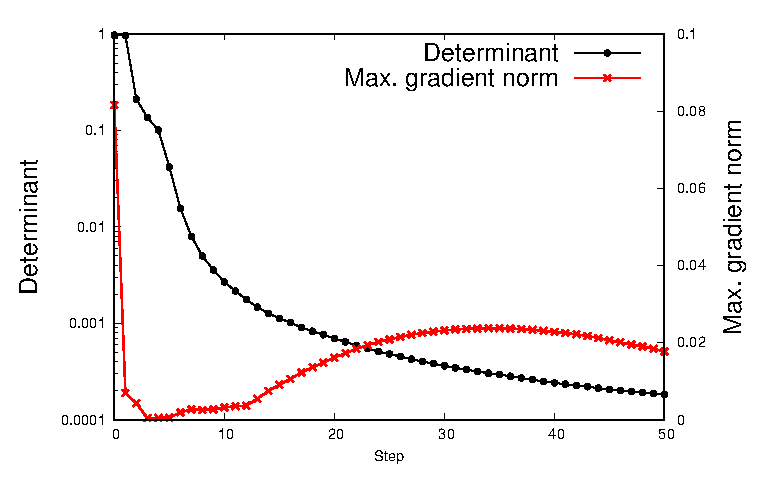
\includegraphics[width=0.5\textwidth]{det}
\caption{
The determinant of the CLMO overlap matrix, the energy, and the maximum norm of the energy gradient with respect to the CLMO coefficients in a direct iterative optimization with the conjugate gradient algorithm. 
Linear system of four hydrogen fluoride molecules interacting through hydrogen bonds is described at the PBE/DZVP level of theory. 
CLMOs of a molecule are allowed to delocalize only over the two nearest neighbors. 
The zero energy is set at the energy of the fully delocalized state. 
For the CLMO state, the energy plateaus even though the gradient does not vanish. 
For the reference, the maximun norm of the gradient of same optimization using fully delocalized orbitals is also shown. %, and converges below $\| \nabla E \|_{\text{max}} < 10^{-6}$~a.u. within 10 iterations.
}
\label{fig:det}
\end{figure}

Substantial efforts have been made to mitigate these problems. 
They include the introduction of an extra set of variational parameters~\cite{yang1997absolute,burger2008linear, peng2013effective} or the energy functionals that can be calculated without inverting the CLMO overlap matrix~\cite{mauri1993orbital,kim1995total,ordejon1995linear}. 
However, despite notable progress~\cite{fattebert2004linear, fattebert2006linear, osei2014accurate} the existing CLMO-based DFT algorithms establish convergence by measuring the rate of change of the energy in the course of the self-consistent field (SCF) procedure and require multiple steps to reach the final state. 
Furthermore, the SCF convergence has not been demonstrated using the norm of the gradient of the energy with respect to the CLMO coefficients -- a much stronger convergence criteria that rules out a possibility of a sluggish optimization illustrated in Figure~\ref{fig:det}.

Importantly, the convergence problem has been reliably solved for weakly-interacting molecular systems. 
It has been shown that CLMOs can be optimized efficiently only if they are forced to be orthogonal to a set of auxiliary tightly localized nonoverlaping orbitals, precomputed and fixed on their molecules~\cite{tsuchida2007augmented, tsuchida2008ab, khaliullin2013efficient}. 
As will be discussed below, this approach works only when the auxiliary orbitals resemble the final variationally optimal CLMOs and thus cannot be applied to finite-gap systems with strong covalent bonds between atoms. 

In this work, a detailed analysis of the origins of the convergence problem enabled us to develop a new linear-scaling CLMO-based DFT method that converges fast for systems of strongly interacting atoms and avoids collapsed states. The proposed method is conceptually simple and does not require any precomputed tightly-localized orbitals nor the optimization of auxiliary variables. These features greatly reduce its computational cost and make it straightforward to implement. Several tests in this work demonstrate the accuracy and efficiency of the method for systems with finite band gap. It is important to state, however, that this method is not expected to be practical for metals and semimetals.

%\begin{itemize}
%\item The energy converges fast, and works with systems where interactions are strong.
%\item The problem of orbital collapse is avoided. 
%\item Conceptually simple and does not require a precomputed reference~\cite{tsuchida2007augmented, khaliullin2013efficient} nor the optimization of auxiliary variables.
%\item Weakness: Although this method is not fully variational and the energy is not the minimum of any energy functional, it still produces stable dynamics for systems involving chemical reactions. Is not expected to be efficient for semimetals and metals.
%\end{itemize}


\section{Theory} 

\subsection{Formalism, notation and main assumptions}
 
%In any CLMO method, concepts of electron \emph{localization centers}, often also referred to as fragments, and electron \emph{localization domains} play key roles. 
In the first step, all atomic nuclei of a system, its electrons, and atom-centered basis set orbitals (AOs) --- in our case Gaussian functions --- are logically divided into nonoverlapping subsets called \emph{localization centers}, often referred to as \emph{fragments}. 
For a system with clearly defined molecules, a typical localization center includes all nuclei of a single molecule, associated AOs and electrons. 
For systems that cannot be partitioned into molecules --- the subject of this work --- a localization center can be represented by a single nuclei. 
As a results of the partitioning, each electron acquires a localization-center label. 
Within Kohn-Sham DFT, electrons are described by molecular orbitals (MOs) \ket{\psi_{xi}} whose indices now indicate that orbital $i$ belongs to center $x$. Throughout this work, centers are labeled with Latin letters $x,y,z$ whereas Latin letters $i,j,k$ label MOs. 

In the next step, each atom $A$ is assigned a predefined element-specific radius $R_c(A)$ that defines neighbors of each center in an obvious way: two centers are considered neighbors if there are atoms located within a sum of their radii. 
\emph{Localization domain} for each center is defined as a subset of AOs that are localized on the neighbors of a center \ket{\chi_{\bar{x}\mu}}. In our notation, index $\bar{x}$ refers to center $x$ and its neighbors. Basis set orbitals are denoted with Greek letters $\mu,\nu,\lambda, \kappa$. 

The basis set orbitals of a localization domain form a subspace in the one-electron vector space and the following projection operator serves as the identity operator on the subspace:
%
\bea
\op{I}_{\bar{x}} = \ket{\chi_{\bar{x}\mu}} S^{\bar{x}\mu,\bar{x}\nu} \bra{ \chi_{\bar{x}\nu}},
\eea
%
where $S^{\bar{x}\mu,\bar{x}\nu}$ is a matrix element of the inverse overlap matrix $S_{\bar{x}\mu,\bar{x}\nu} = \braket{ \chi_{\bar{x}\mu}}{ \chi_{\bar{x}\nu}} $. Note that the conventional tensor notation is used to work with the nonorthogonal orbitals~\cite{head1998tensor}: covariant quantities are denoted with subscripts, contravariant quantities with superscripts, and summation is implied over the same orbital indices but not over the same center and domain indices. 

By construction a basis set function may belong to several localization domains or, in other words, domains often overlap. 

In the final step, the main approximation of CLMO methods is introduced. It is assumed that the electronic structure of the system can be described accurately by molecular orbitals that are completely localized within domains of their centers
%
\bea
\ket{\psi_{xi}} = \op{I}_{\bar{x}} \ket{\psi_{xi}}
\label{eq:LMO}
\eea
%
Thus this approximation imposes a blocked structure on the matrix of MO coefficients
\bea
\ket{\psi_{xi}} = \ket{\chi_{\bar{x}\mu}} {T^{\bar{x}\mu}}_{xi}.
\label{eq:LMOproj}
\eea
%
The size of blocks is determined entirely by the pre-selected $R_{c}$ and does not change with the number of molecules. Therefore, in the limit of large systems, the computational cost of the optimization grows linearly with the number of atoms offering a way of performing LS calculation directly with MOs. % RZZK: comment how accurate this apprx is expected to be for finite-gap and metallic systems.  

In this work, we consider only spin-unpolarized orbitals evaluated at the $\Gamma$-point. The KS DFT energy functional can be written in the conventional way 
% RZZK check the equation
\bea
E &=& 2 \trace \left[ \op{R} \op{H} \right] - \frac{1}{2} \int\int \frac{\rho(\br)\rho(\br')}{|\br-\br'|}d\br d\br' \nonumber \\
 &+& E_{\text{XC}} - \int v_{\text{XC}}(\br) \rho(\br) d\br,
\eea
%
where \op{H} is the Kohn-Sham Hamiltonian, \op{R} is the projection operator onto the occupied subspace, and $\rho(\br) = 2\bra{\br}\op{R}\ket{\br}$ is the electron density. \op{R} written to take into account the nonorthogonality of CLMOs
\bea \label{eq:dm}
\op{R} = \sum_{x,y} \ket{\psi_{xi}} \sigma^{xi,yj} \bra{\psi_{yj}},
\eea
%
where $\sigma^{xi,yj}$ is a matrix element of the inverse of the CLMO overlap matrix $\sigma_{zk,xj} = \braket{ \psi_{zk}}{ \psi_{xj}} $.

\subsection{Convergence problem and Hessian eigenspectrum}

The direct minimization of the energy functional with respect to molecular orbital coefficients is a straightforward reliable low-cost method optimization for fully delocalized orbitals ($R_c \rightarrow \infty$)~\cite{galli1992large, vandevondele2003efficient, van2002geometric} and completely localized orbitals ($R_c = 0$)~\cite{khaliullin2013efficient}. 
% voorhis2002geometric - https://doi.org/10.1080/00268970110103642
The preconditioned conjugate gradient algorithm (PCG) is a particularly efficient energy minimizer that requires iterative evaluation of the energy gradient
%
\bea \label{eq:grad}
{G_{\bar{x}\mu}}^{xi} \equiv \frac{\partial E}{\partial {T^{\bar{x}\mu}}_{xi}} = 4 \bra{\chi_{\bar{x}\mu}} (\op{I}-\op{R}) \op{H} \ket{\psi^{xi}}
\eea
%
and only a single inversion of a preconditioner. The latter is typically chosen as an easily-invertible approximation to the exact Hessian. It has been found~\cite{vandevondele2003efficient,khaliullin2013efficient} that, for the two special cases $R_c \rightarrow \infty$ and $R_c = 0$, the preconditioner defined on domain $\bar{x}$
%
\bea \label{eq:prec}
P_{\bar{x}\mu,\bar{x}\nu} &=& 4 \bra{\chi_{\bar{x}\mu}} (\op{I}-\op{R}) (\op{I} + \op{H})(\op{I}-\op{R}) \ket{\chi_{\bar{x}\nu}} 
\eea
%
provides the same rate of convergence of the PCG algorithm as the exact Hessian but at a fraction of the inversion cost. The relation between the preconditioner in Eq.~(\ref{eq:prec}) and the exact Hessian is presented in the Supplementary Material. 

\begin{figure*}
\centering
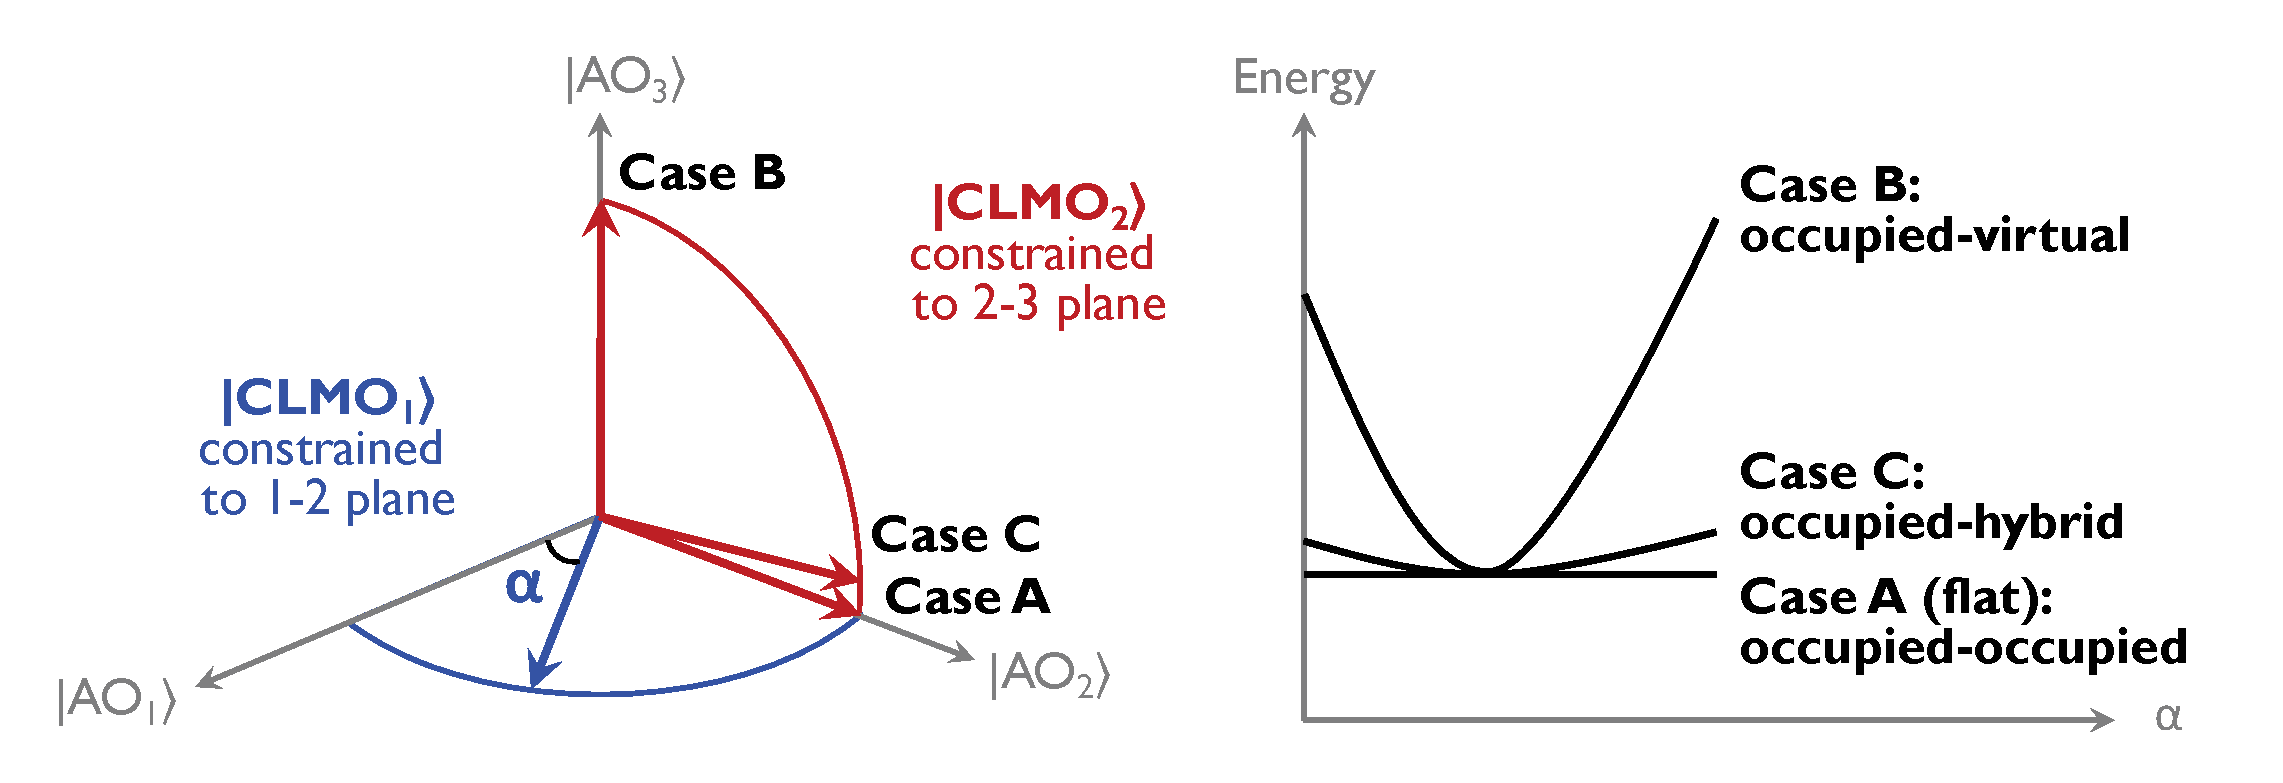
\includegraphics[width=0.75\textwidth]{modes}
\caption{Illustration of the origin of low-curvature modes in a model vector space spanned by three basis set functions \ket{\text{AO}_1}, \ket{\text{AO}_2}, \ket{\text{AO}_3}. The left panel shows \ket{\text{CLMO}_1} (blue) confined to its domain spanned by \ket{\text{AO}_1} and \ket{\text{AO}_2} as well as \ket{\text{CLMO}_2}  (red, three cases) confined to its domain spanned by \ket{\text{AO}_2} and \ket{\text{AO}_3}. The right panel shows the behavior of the energy as a function of the position of \ket{\text{CLMO}_1} --- angle $\alpha$ --- for three typical cases. Case C shows that the low-curvature modes arise when \ket{\text{CLMO}_2}  lies almost entirely in the domain of \ket{\text{CLMO}_1}.}
\label{fig:modes}
\end{figure*}

In the general case of finite $R_c$, the PCG-based optmization of CLMOs has been investigated thoroughly as a low-cost alternative to LS DM-based DFT methods~\cite{mauri1993orbital, kim1995total, ordejon1995linear, fattebert2004linear, fattebert2006linear, burger2008linear, peng2013effective, khaliullin2013efficient}. 
This approach is expected to be very efficient because both the CLMO coefficient and gradient matrices are small (i.e. number of columns is much smaller then the number of rows) and enforced to be sparse. 
In addition to this, the inversion of the approximate Hessian in Eq.~\ref{eq:prec} can be done fast, domain-by-domain. 
%
Unfortunately, the PCG algorithm, as well as all other optimization procedures (e.g. Newton-Raphson or DIIS-accelerated diagonalizations)~\cite{stoll1980use}, suffer from the aforementioned slow convergence and orbital collapse problems. 
%
A closer inspection of the eigenvalues of the preconditioner obtained by solving the generalized eigenproblem for each domain 
%
\bea
P_{\bar{x}\mu,\bar{x}\nu} {A^{\bar{x}\nu}}_{xp} =  S_{\bar{x}\mu,\bar{x}\lambda} {A^{\bar{x}\lambda}}_{xp} \Lambda_{xp},
\label{eq:gev}
\eea
%
reveals the origin of this and other closely related previously reported problems~\cite{goedecker1999linear}. 
The eigenvalues, which approximate the energy curvature along the optimization direction \ket{d_{xp}} given by the corresponding eigenvector, ${A^{\bar{x}\nu}}_{xp} \equiv \braket{\chi^{\bar{x}\nu}}{d_{xp}}$, can be divided into three categories according to their magnitudes. 
Zero eigenvalues in the first category represent optimization directions towards occupied orbitals localized completely within the same domain (Figure~\ref{fig:modes}, case A). 
As expected the energy is invariant along these occupied-occupied mixing modes. 
The second category includes large nonzero eigenvalues that represent the optimization in the direction toward unoccupied orbitals (Figure~\ref{fig:modes}, case B) of the domain. 
These two categories are the only present in the rapidly converging optimization of fully delocalized orbitals ($R_c \rightarrow \infty$) and absolutely localized orbitals ($R_c = 0$). 
The eigenvalues classified as the third category are extremely small but nonzero (Figure~S1 in the Supplementary Material). 
They appear only for finite $R_c$ when domains share basis set functions. 
The optimization along these low-curvature nearly-invariant directions is difficult to converge because various analytical approximations (e.g. approximate Hessian, quadratic linear search) and numerical noise (e.g. finite DFT grids) make calculations  imprecise. 
In other words, optimization with finite $R_c$ becomes ill-conditioned and the low-curvature modes represents the major barrier to the practical use of promising orbital-based LS DFT methods. 

\section{Results and discussion}

\subsection{Nature of low-curvature modes} \label{marker:nature} 

What is the physical origin of the low-curvature optimization modes? 
It has been suggested previously~\cite{goedecker1999linear} that the sluggish optimization in orbital-based LS DFT is due to the inexact invariance of the energy with respect to the mixing of occupied orbitals. 
Although this might indeed present a problem for a series of functionals based on DMs that are not fully idempotent~\cite{mauri1993orbital,kim1995total,ordejon1995linear} the DM used in this work is constructed with the inverse of the overlap matrix and, therefore, is properly idempotent and exactly invariant to the mixing among occupied states. 

We instead suggest that the low-curvature optimization modes represent \emph{hybrid} directions, which are neither occupied nor virtual. From the point of view of the local vector subspace of $\bar{x}$, these directions exist because CLMOs of neighbor centers are only partially localized on $\bar{x}$. 
Hybrid directions, originating from CLMOs that are almost but not entirely localized on the domain, are expected to be particularly problematic (Figure~\ref{fig:modes}, case C). 


%Our hypothesis can be verified by calculating the residue $\Delta$ of the small-curvature directions \ket{d_{\bar{x}p}} in the unoccupied space projected onto subspace of a domain:
%
Our hypothesis implies that a hybrid low-curvature mode $\ket{d_{\bar{x}p}}$ has only small component in the unoccupied subspace of domain $\bar{x}$. 
This component is measured by the residue $\Delta_{\bar{x}p}$ 
\bea
\label{eq:residue}
\Delta_{\bar{x}p} \equiv \bra{d_{\bar{x}p}} \op{I}_{\bar{x}} - \op{R}_{\bar{x}} \ket{d_{\bar{x}p}}, 
\eea
%
where $\op{R}_{\bar{x}}$ is a projector constructed from the occupied CLMOs of the neighbors truncated to the subspace $\bar{x}$ with operator $\op{T}_{\bar{x}} \approx \op{I}_{\bar{x}}$
\bea
\op{R}_{\bar{x}} &=& \sum_{y,z \in \bar{x}} \op{T}_{\bar{x}} \ket{\psi_{yi}} \sigma_{\bar{x}}^{yi,zj} \bra{\psi_{zj}} \op{T}_{\bar{x}}
%R^{\bar{x}\mu,\bar{x}\nu} &\equiv& \bra{\chi^{\bar{x}\mu}} \op{R}_{\bar{x}} \ket{\chi^{\bar{x}\nu}} \\
\label{eq:C}
\eea
%
and $\sigma_{\bar{x}}$ is the overlap matrix of the truncated orbitals. 
%%
%\bea
%\left(\sigma_{\bar{x}}\right)_{yi,zj} = \bra{\psi_{yi}} \op{I}_{\bar{x}} \ket{\psi_{zj}}
%\eea
%%

Figure~\ref{fig:projection} shows that the small-curvature modes indeed lie mostly outside the unoccupied space for a variety of materials (see Supplementary Material for details). 
It is also interesting to note that the unoccupied fraction of the low-curvature modes increases with the strength of interatomic delocalization (i.e. the degree of covalency of bonding). 

Thus the optimization along the low-curvature modes of a domain represents mixing of its occupied CLMO with the occupied orbitals of its neighbors that are not fully localized on the domain. 
Unsurprisingly, such orbital variations often lead to linear dependencies among occupied orbitals and eventual collapse of the optimization. 

\begin{figure}
\centering
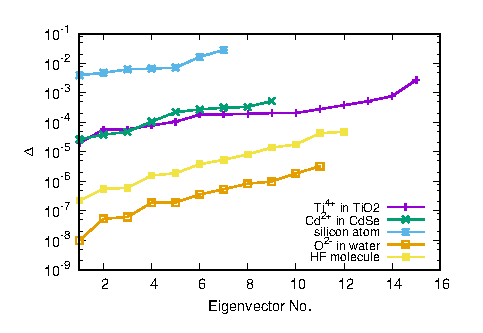
\includegraphics[width=0.5\textwidth]{residue}
\caption{
The norm of the projection of the small-curvature modes on the unoccupied subspace of a domain. 
Preconditioner eigenvectors with the eigenvalues smaller than 0.02~a.u. are chosen as small-curvature modes. 
The following localization ceneters are considered: Ti$^{4+}$ ions in the TiO$_2$ rutile lattice, Cd$^{2+}$ ions in the CdSe Wurtzite lattice, Si atom in the diamond silicon lattice, O$^{2-}$ in a water tetramer system, hydrogen fluoride molecule in a linear tetramer system. 
The BLYP/TZV2P level of theory is used for water and PBE/DZVP in all other tests.}

\label{fig:projection}
\end{figure}

The proposed explanation of the nature of the low-curvature modes is consistent with the fact that, for molecular partitioning, the number of the low-curvature modes is equal to the sum of occupied orbitals on the neighbor fragments. It also explains why the two-stage procedure of Ref.~\onlinecite{khaliullin2013efficient} works so well for molecular systems. In the first stage of this procedure, $R_c$ is set to zero and the resulting block-diagonal orbitals \ket{\psi_{xi}^{0}} are optimized variationally to construct the occupied space projector $\op{R}^{0}$. This projector is then fixed, $R_c$ is reset to its original finite value to allow intercenter electron delocalization, and the following trial orbitals are optimized with respect to CLMOs coefficients:
%
\bea
\ket{\psi_{xi}} &=& \ket{\psi_{xi}^{0}} + \op{I}_{\bar{x}} (\op{I} - \op{R}^{0} ) \ket{\chi_{\bar{x}\mu}} \bar{T}^{{\bar{x}\mu}}_{xi}
\eea
%
For these CLMOs, the gradient and preconditioner
%
\bea \label{eq:grad-bar}
\bar{G}{_{\bar{x}\mu}}^{xi} &\equiv & \frac{\partial E}{\partial \bar{T}^{{\bar{x}\mu}}_{xi}} = 
%4 \bra{\chi_{\bar{x}\mu}} \op{Q}_{\bar{x}}^{0} (\op{I}-\op{R}) \op{H} \ket{\psi^{xi}} = \nonumber \\
%&=& 
\bra{\chi_{\bar{x}\mu}} \op{Q}_{\bar{x}}^{0} \ket{\chi^{\bar{x}\nu}} {G_{\bar{x}\nu}}^{xi}
\eea
%
\bea \label{eq:prec-bar}
\bar{P}_{\bar{x}\mu,\bar{x}\nu} &=& 
%\bra{\chi_{\bar{x}\mu}} (\op{I} - \op{R}^{0} ) \ket{\chi^{\bar{x}\lambda}}  P_{\bar{x}\lambda,\bar{x}\kappa} \bra{\chi^{\bar{x}\kappa}} (\op{I} - \op{R}^{0} ) \ket{\chi_{\bar{x}\nu}}
\bra{\chi_{\bar{x}\mu}} \op{Q}_{\bar{x}}^{0} \ket{\chi^{\bar{x}\lambda}}  P_{\bar{x}\lambda,\bar{x}\kappa} \bra{\chi^{\bar{x}\kappa}} \op{Q}_{\bar{x}}^{0} \ket{\chi_{\bar{x}\nu}}
\eea
%
are related to those in Eqs.~(\ref{eq:grad}) and~(\ref{eq:prec}) via domain-specific projectors
%
\bea \label{eq:q0}
\op{Q}_{\bar{x}}^{0} &\equiv & \op{I}_{\bar{x}} (\op{I} - \op{R}^{0} ) \op{I}_{\bar{x}}
\eea
%

As shown in Ref.~\onlinecite{khaliullin2013efficient}, projector $\op{Q}_{\bar{x}}^{0}$ is key to converge orbital optimization for molecular systems. The present work explains that this is because $\op{Q}_{\bar{x}}^{0}$ satisfies two important requirements. First, it is constructed from CLMOs fully localized on their centers. This ensures that each domain contains an integer number of occupied dimensions. Second, it is constructed from $\op{R}^0$ that is already close to the final converged DM. This, therefore, guarantees that $\op{Q}_{\bar{x}}^{0}$ removes the low-curvature optimization modes.  

Unfortunately, the two-stage approach does not work for systems with strong covalent bonds between localization centers (i.e. atoms). This is illustrated in Figure~\ref{fig:convergence} for the cadmium selenide lattice. The main reason for the deteriorating convergence is the inability of $\op{R}^0$, which is constructed from the block-diagonal CLMOs, to adequately represents the low-curvature modes in the delocalized states encountered in later stages of the optimization. 

\begin{figure}
\centering
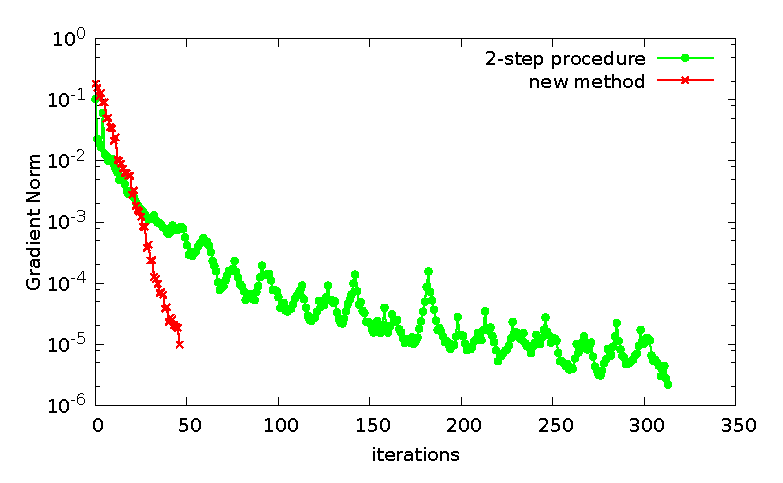
\includegraphics[width=0.5\textwidth]{convergence}
\caption{The maximun norm of the energy gradient for the PBE/DZVP basis~\cite{vandevondele2007gaussian} optimization of the CLMOs for the hexagonal wurtzite CdSe lattice. $R_c = 3.5$~{\AA}. Modes with the preconditioner eigenvalues lower than 0.05~a.u. are removed from the optimization. The block-diagonal projector is described in Eq.~\ref{eq:q0}.} 
%The difference in the ground state energy for the two methods is 0.03 kJ/mol per Cd atom.
\label{fig:convergence}
\end{figure}


\subsection{Proposed solution to the optimization problem}

We propose to solve the convergence problem by detecting the low-curvature modes directly by diagonalizing the approximate Hessian in Eq.~(\ref{eq:prec}) and avoiding the optimization along these modes altogether. Although this procedure does not produce fully optimized orbitals they are still expected to provide accurate representation of the ground state. This is because the low-curvature modes are associated mostly with mixing of occupied and nearly-occupied orbitals and, therefore, are expected to be \emph{shallow} optimization directions. That is, they are unlikely to produce a noticeable variational decrease in the energy.

To filter out the low-curvature modes we construct a projector
%
\bea
%L^{\bar{x}\mu,\bar{x}\nu} &=& {A^{\bar{x}\mu}}_{xp} \Theta_{xp} {A^{\bar{x}\nu}}_{xp} \\
\op{Q}_{\bar{x}} &=& \ket{d_{\bar{x}p}} \, \Theta\left[ \Lambda_{\bar{x}p} - \Lambda_c \right] \bra{d_{\bar{x}p}},
\eea
%
where \bra{d_{\bar{x}p}} are eigenvectors of the approximate Hessian from Eq.~(\ref{eq:gev}) and $\Theta$ is the unit step function 
\bea
\Theta \left[\Lambda_{\bar{x}p} - \Lambda_c \right] =
\begin{cases} 
      0 & \Lambda_{\bar{x}p} \leq \Lambda_c ,\\
      1 & \Lambda_{\bar{x}p} \geq \Lambda_c
\end{cases}
\eea
%
and $\Lambda_c$ is the curvature threshold below which the optimization mode is classified as a low-curvature mode. This projector is then applied to the gradient and preconditioner in the PCG optimization algorithm
%
\bea
\tilde{G}{_{\bar{x}\mu}}^{xi} &=& \bra{\chi_{\bar{x}\mu}} \op{Q}_{\bar{x}} \ket{\chi^{\bar{x}\nu}} {G_{\bar{x}\nu}}^{xi} \label{eq:grad-lcp} \\
%
\tilde{P}_{\bar{x}\mu,\bar{x}\nu} &=& \bra{\chi_{\bar{x}\mu}} \op{Q}_{\bar{x}} \ket{\chi^{\bar{x}\lambda}}  P_{\bar{x}\lambda,\bar{x}\kappa} \bra{\chi^{\bar{x}\kappa}} \op{Q}_{\bar{x}} \ket{\chi_{\bar{x}\nu}} \label{eq:prec-lcp}.
\eea
%
As a result, the PCG optimization procedure neglects the low-curvature modes. 
%Hopefully, the energy changes associated with them are  small. 

We will refer to the new method based on Eqs.~(\ref{eq:grad-lcp}) and (\ref{eq:prec-lcp}) as low-curvature projector (LCP) method.
%RZZK- this would be a good place to say a couple of words about the connection of LCP to the two-stage procedure, its trial CLMOs and its weaknesses: dependence on optimization path, absence of a well-defined trial wavefunction.
%Use this?: We note that upon applying the LCP $\op{Q}_{\bar{x}}$ on the gradient, the final energy is no longer fully variational: the gradient is only zero in diretions that significantly change the energy. It also implies that the energy will depend on the optimization path.

%RZZK: Add to discussion: One weakness of defining CLMO domains \emph{a priori} in this way is that at least rough idea about the electron distribution in a system is required to assign electrons to localization centers and domains. Such a procedure is, of course, not applicable to systems in which the exact bonding properties are unknown.

%RZZK: Discuss advantages and weaknesses of the new method: (a) We are giving up a strict energy functional. As a consequence, the final energy may depend on the optimization path (i.e. how often the PCG is restarted and preconditioner is recalculated). However, we demonstrate that the dependence of the energy on optimization path is insignificant and the final energy is close to the ground state. Moreover, the proposed method passes even more stringent test: it appears to produce stable molecular dynamics trajectories. As stated before, the filtered directions should be primarily occupied-occupied mixing, so that physically meaning full directions are not neglected and the final state is close to the true ground state. 

%RZZK: The physical meaning of Eq~\ref{eq:approxq} is a modified orthogonality constrain for LMOs. Orthognality and locality has generally been considered as competing properties: strict orthogonality leads to decaying tails, and for LMOs no orthogonality constrains are imposed except for MOs within a fragment. However, this causes the convergence problem previously mentioned: LMOs without orthogonality tends to collapse. Although global orthogonality cannot be achieved, we suggest a local orthogonality constrain, that the projection of MOs onto each fragment $x$ should be orthogonal. Unlike the case for none-local MOs, not every physical state can be transformed into such state.

%RZZK: While many previous works~\cite{RZZK} dealt with weakly-interacting fragments (e.g. molecules) the approach here represents the ultimate atomic partitioning scheme.

\subsection{Implementation}

The procedure for finding and projecting out the low-curvature modes is implemented in the CP2K software package~\cite{www:cp2k}. CP2K relies on the mixed Gaussian and plane wave representation of the electronic degrees of freedom~\cite{vandevondele2005quickstep} and is an ideal platform for the new orbital-based LS method: just a few tightly-localized Gaussian AOs can provide an accurate representation of CLMOs, whereas plane waves ensure a fast LS construction of the KS Hamiltonian for large systems.

All matrix multiplications are performed with the DBCSR library~\cite{borvstnik2014sparse} designed for massively-parallel linear-scaling handling of large sparse matrices. 
A special care is taken to reduce the computational overhead of the optimization procedure for large Gaussian basis sets. 
To this end, the order of matrix multiplications in Eqs.~(\ref{eq:grad-lcp}) and (\ref{eq:prec-lcp}) is chosen to avoid steps that scale cubically with the size of the Gaussian basis set. 
The diagonalization of the preconditioner matrices is done independently for each domain. 

It is important to note that the construction of the DM requires the inversion of the CLMO overlap matrix. 
This matrix is small and its size is independent of the size of the basis set. 
However, it is not confined to individual domains. This inversion is carried out using the iterative Hotelling method~\cite{hotelling1943some} that is based entirely on matrix multiplications and becomes LS when the system is large and the CLMO overlap and its inverse are sparse. 

Because of the similarity between the new method and the ALMO SCF for molecular systems only minor modifications in the existing ALMO DFT module of CP2K are necessary. The main difference between the algorithms in the two approaches is that the PCG optimization of CLMOs in the LCP method might need more frequent re-evaluation and inversion of the preconditioner.

%RZZK: PCG is restarted once in a while or it can be restarted quite often. If it is restarted and precond is evaluated on every step it become a Newton-Raphson with approximate Hessian.

\subsection{Accuracy and efficiency tests}

%\subsection{Convergence}

Figure~\ref{fig:convergence} shows that the new optimization procedure converges rapidly for the hexagonal CdSe lattice -- a particularly challenging case for LS methods considering the small band gap of this material and strong interactions between atoms. 
In contrast, it is difficult to achieve convergence for this system using the two-stage method described in Ref.~\cite{khaliullin2013efficient}. 
It is also important to note that the final energy obtained with the new method differs from the energy obtained after 250 iterations  of the unconverged two-stage procedure only by 0.03 kJ/mol per Cd atom. 

%\subsection{Accuracy} 

The accuracy of the LCP energies as a function of $R_c$ is shown in Figure~\ref{fig:accuracy} for several challenging systems with strong interaction and significant electron delocalization between fragments: CdSe in the hexagonal wurtzite lattice; liquid water in which each atom is treated as a fragment; silicon in the cubic diamond lattice. 
Figure~\ref{fig:accuracy} demonstrates that the energy converges to the correct ground state energy as $R_c$ increases. The error of the localization constraints imposed on electrons is small. The insets in Figure~\ref{fig:accuracy} also shows that the error of projecting out the low-curvature optimization modes is even smaller than that introduced by finite $R_c$. These tests confirm our hypothesis that the low-curvature directions do not produce a noticeable decrease in the energy.

\begin{figure}
\centering
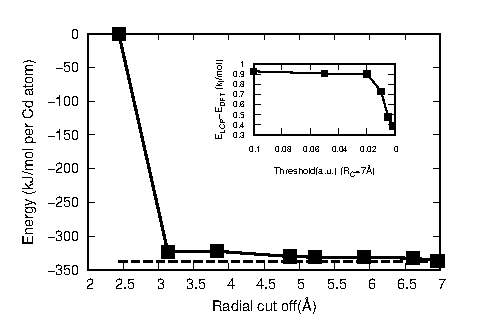
\includegraphics[width=0.35\textwidth]{CdSe_conv}
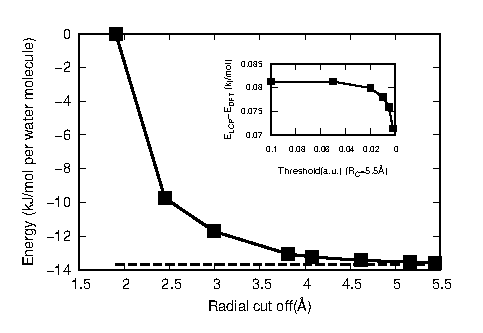
\includegraphics[width=0.35\textwidth]{H2O_conv}
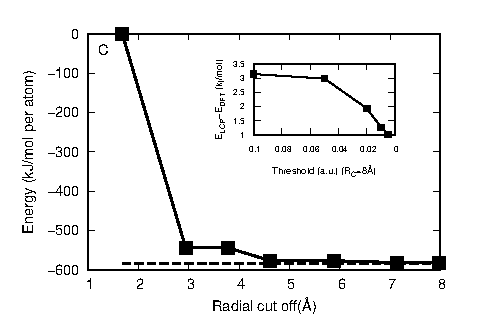
\includegraphics[width=0.35\textwidth]{Si_conv}
\caption{Energy from the low-curavture projector and the dependence on the localization radii $R_c$ for: A. PBE/DZVP calculation for the hexagonal wurtzite phase of CdSe, B. BLYP/TZV2P calculation for atomically-partitioned liquid water, C. PBE/DZVP calculation for the cubic diamond phase of silicon. The convergence criteria is $\vert\vert \tilde{G} \vert\vert_{\text{max}} < 10^{-5}$~a.u. The zero energy is set at the energy of the fully optimized block-diagonal CLMOs (R$_c = 0$). Dashed line shows the reference energy of conventional DFT calculation (E$_{\text{DFT}}$) without localization constrains (R$_c\rightarrow \infty$). 
Inset: LCP energy dependence on the low-curvature threshold $\Lambda_c$ at a fixed $R_c$. For the inset, the energy of the unconstrained orbitals is chosen as zero.}
\label{fig:accuracy}
\end{figure}

To demonstrate the accuracy of the LCP energies further, we performed a 500~K Monte Carlo (MC) simulation of silicon in the cubic diamond lattice with a defect created by replacing two neighboring silicon atoms with two carbon atoms. Figure~\ref{fig:mc} shows that the silicon-silicon radial distribution function (RDF) at equilibrium almost perfectly reproduces that calculated using conventional DFT methods for fully delocalized electrons. 

\begin{figure}
\centering
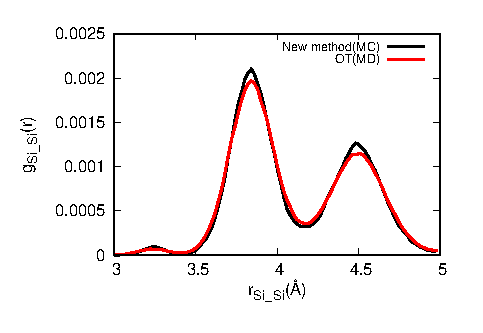
\includegraphics[width=0.45\textwidth]{rdf_si}
\caption{Silicon-silicon RDF calculated for the cubic diamond phase of silicon with carbon atoms introduced to create a point defect. XC/basis simulations are performed at $T=500$~K with the conventional orbital-transformation~\cite{vandevondele2003efficient} method for the delocalized electrons and the LCP method with $R_c = 6$~\AA\ and $\Lambda_c = 0.02$~a.u. The system includes 62 silicon atoms and two carbon atoms.}
\label{fig:mc}
\end{figure}

%\subsection{Stable molecular dynamics simulations}

Molecular dynamics (MD) simulations present an even more stringent test on the accuracy of the LCP method. While minor energy errors are not crucial in fixed-nuclei calculations, geometry optimizations, and Monte-Carlo sampling they tend to accumulate in MD trajectories leading to non-physical sampling and eventual failure of simulations. Accurate calculation of forces is therefore crucial for molecular dynamics simulations, the stability of which are judged by the accumulated drift in the conserved quantity (e.g. total energy of the system). Although CLMOs obtained with the LCP method are not strictly variational we chose to neglect this error and invoke the Hellmann--Feynman theorem~\cite{feynman1939forces} in the calculation of atomic forces. This procedure is then used to perform an LCP-based MD simulation of a protonated water nanocluster containing 62 water molecules and two protons. In the course of a three-picosecond MD simulation, the two protons hop around breaking and forming covalent bonds with water molecules. To reproduce motion of protons around the nanodroplet each atom was treated as a localization center. Setting $R_c = 4$~\AA\ and $\Lambda_c = 0.005$~a.u. produces sufficiently optimized CLMOs to ensure the stability of the MD simulation. Figure~\ref{fig:md} shows that the drift in the conserved quantity is acceptably small compared to the magnitude of the fluctuations in the potential energy. The applicability of the LCP method in MD simulations will be explored further especially in conjunction with the modified Langevin integrator method~\cite{scheiber2018communication}. 

\begin{figure}
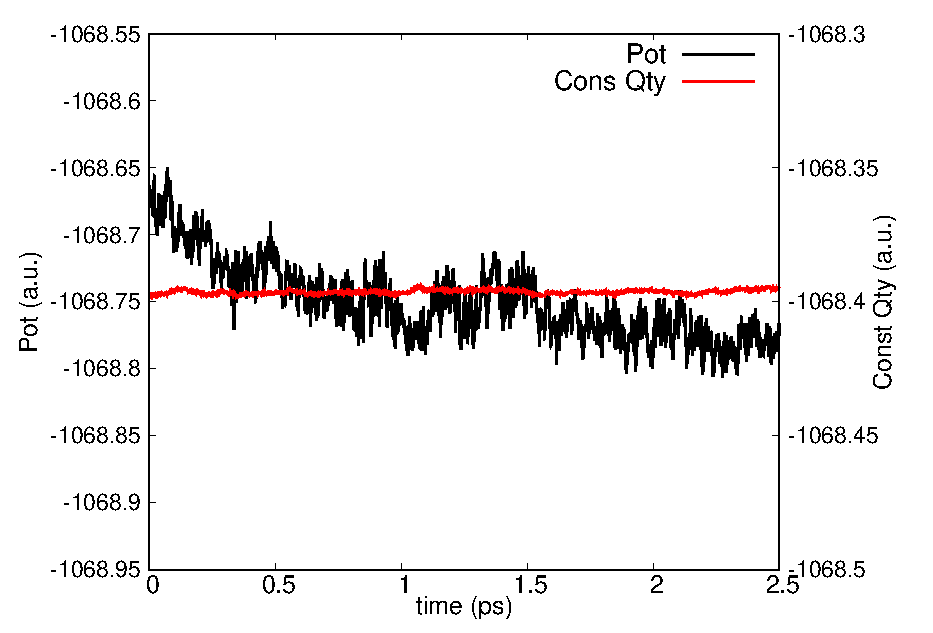
\includegraphics[width=0.45\textwidth]{const.eps}
\caption{The potential energy and the conserved quantity in a LCP-based MD simulation of a protonated water nanocluster $\text{(H}^{+}\text{)}_2\text{(H}_2\text{O)}_{62}$. The temperature of the NVT simulations is set to 298~K and controlled by a canonical velocity re-scaling thermostat~\cite{bussi2007canonical} with the coupling time constant of 50~fs. The potential energy and conserved quantity are shifted for clarity.}
\label{fig:md}
\end{figure}


%\subsection{Computational efficiency}

To test the computational efficiency of the newly designed method, we compared its performance to the orbital transformation (OT) method~\cite{weber2008direct,vandevondele2003efficient} --- a well-optimized low-prefactor cubic scaling DFT method for conventional fully delocalized orbitals. The calculation is done for the hexagonal CdSe system of different sizes. $R_c$ is set to 3.5~{\AA}, which is large enough to accurately describe the electronic structure of the system (Figure~\ref{fig:accuracy}) and $\Lambda_c = 0.02$~a.u. Figure~\ref{fig:scaling} demonstrates that the LCP method is asymptotically LS. The LS regime is achieved when the MO overlap matrix and its inverse are sparse. For a dense 3D system like CdSe it takes on the order of $\sim$3000 atoms. 
% RZK: Do you have timing DM LS timing for a couple of small systems?
% Yiei: EPS_DEFAULT: 1E^-12 EPS_FILTER: 1E-8

\begin{figure}
\centering
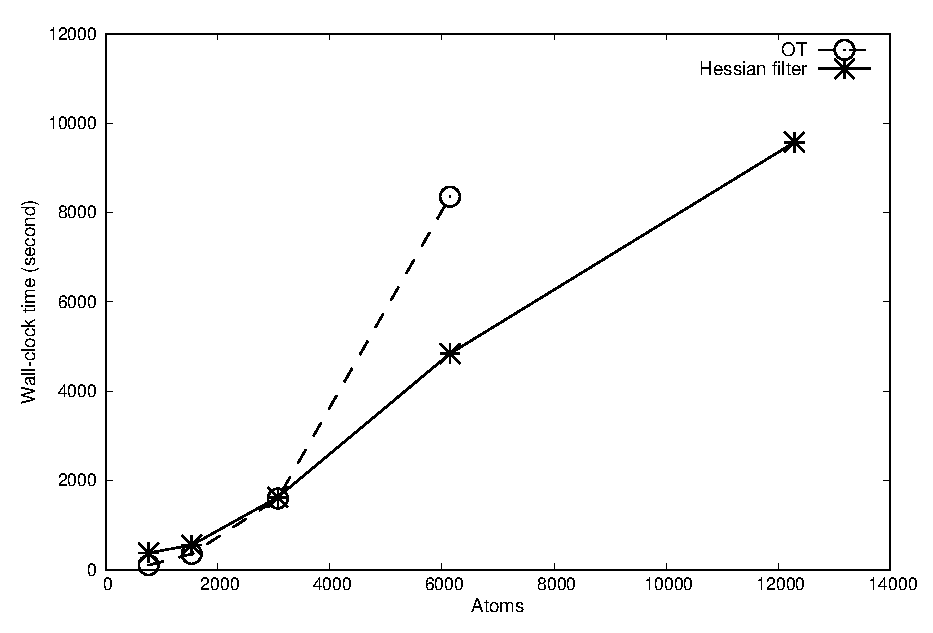
\includegraphics[width=0.45\textwidth]{timing}
\caption{CLMO optimization timing benchmark for the hexagonal CdSe lattice. The PBE/DZVP calculation with $R_c=3.5$~{\AA} and $\Lambda_c = 0.02$~a.u. is done on 256 compute cores. 
}
\label{fig:scaling}
\end{figure}


\section{Conclusions} 

This work presents a new linear-scaling DFT method based entirely on the conceptually simple variational optimization of localized molecular orbitals. 
Unlike many existing LS methods, the method does not perform the typical concomitant variation of the density matrix and thus has low computational cost. 
The notorious convergence problem that has plagued orbital-based LS DFT methods is resolved by avoiding the optimization of orbitals along low-curvature modes -- the directions associated with tiny eigenvalues of the electronic Hessian. 
An efficient procedure is designed to identify the low-curvature modes on-the-fly without the computationally costly construction and diagonalization of the Hessian. 
It is also shown that the low-curvature modes --- an unavoidable repercussion of imposing localization constraints --- can be safely neglected because they are associated with the mixing of nearly occupied states and do not produce a noticeable variational decrease in the energy. 

The new methodology, which is expected to be applicable to systems with nonvanishing band gap, is tested on a variety of materials including rutile phase of titania, hexagonal phase of cadmium selenide, and cubic diamond phase of silicon with and without defects. 
These tests demonstrate that the method is accurate and efficient even when localization centers are represented by single atoms and there are strong covalent interaction between the centers. 
Furthermore, preliminary tests on protonated water nanoclusters suggest that the atomic partitioning does not present problems for the new method and it is sufficiently robust to enable stable molecular dynamics simulation of bond-breaking and formation processes. 

The developed LS DFT method is expected to have a significant impact on computational modeling of complex systems due to its low computational overhead, enabling calculations on previously inaccessible time and length scales and making completely new chemical phenomena amenable to simulations.

\section{Acknowledgments} The research was funded by the Natural Sciences and Engineering Research Council of Canada through the Discovery Grant (RGPIN-2016-05059). The authors are grateful to Compute Canada for computer time.

%RZK: references should be formatted properly. JCTC strongly recommends using achemso style package
\bibliography{negref}

\newpage
\newpage

%Y. Shi and R. Z. Khaliullin ``Robust linear-scaling optimization of compact localized orbitals in density functional theory''

\begin{figure*}
\includegraphics[width=3.5in]{toc.pdf}
\caption{
Table of Contents use only
}
\label{fig:toc}
\end{figure*}


\end{document}
